\documentclass[12pt]{article}

\usepackage[margin=1in]{geometry}
\usepackage{amssymb}
\usepackage{amsmath}
\usepackage{graphicx}
\usepackage{subcaption}

\setlength{\parskip}{1em}


\newenvironment{question}[2][Question]{\begin{trivlist}
\kern10pt
\item[\hskip \labelsep {\bfseries #1}\hskip \labelsep {\bfseries #2.}]}{\end{trivlist}}


\begin{document}

\title{DD2424 Deep Learning in Data Science Assignment 2}
\author{Lin Chun Hung, chlin3@kth.se}

\maketitle

\section{Basic Part (Part 1)}
\begin{question}{i}
Two methods were used to ensure that the analytical gradient computations were bug
free.
They were the sanity check and checking against the numerical gradient methods.

The implementations of these two methods were written in
\texttt{test/test\_2l\_clsr.py} and \texttt{test/test\_ann\_2l.py} respectively.

For the sanity check, the cost function obtained a very low training cost (\texttt{lambda} = 0)
and loss (i.e. $\leq 0.05$).
For the numerical gradient, the step size to \texttt{1e-5} was set and
double precision matrices were used as the cost function in the problem is non-linear.
The numerical results was consistent with the analytical results.

Therefore, it is safe to say that the implementation of the
analytic gradient computations were bug free.
\end{question}

\begin{question}{ii}

The replications of the figure 3 and 4 are plotted in \ref{fig:replicate_f3} and
\ref{fig:replicate_f4}.

In the figure \ref{fig:replicate_f4}, we can see that at update step 1600, 3200,
and 4800 there are local minima. Therefore the model weightings at these minima
can be considered as a ensemble and it is of a cheap cost.
On the other hand, it means we have to
train the network with complete cycle or integer cycles otherwise it will not go to any local
minimum point.

\begin{figure}[!htb]
    \begin{subfigure}[b]{0.32\textwidth}
        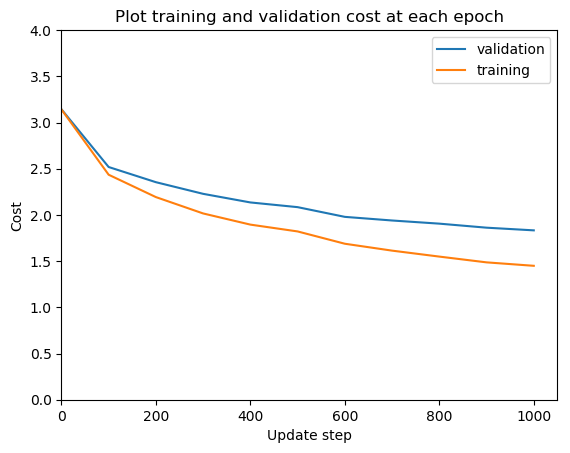
\includegraphics[width=\linewidth]{f3_cost_plt.png}
        \caption{Cost plot}
    \end{subfigure}
    \hfill
    \begin{subfigure}[b]{0.32\textwidth}
        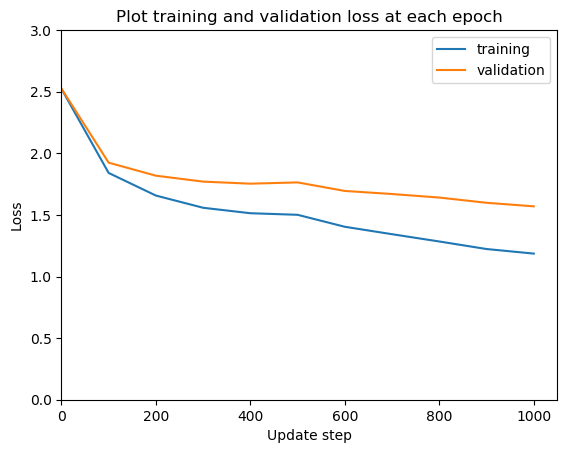
\includegraphics[width=\linewidth]{f3_loss_plt.png}
        \caption{Loss plot}
    \end{subfigure}\hfill
    \begin{subfigure}[b]{0.32\textwidth}%
        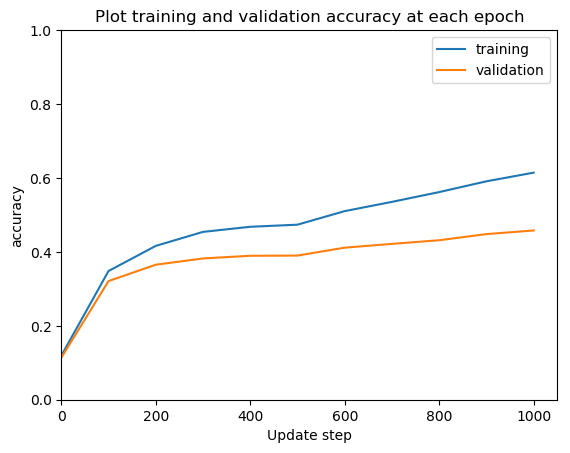
\includegraphics[width=\linewidth]{f3_acc_plt.png}
        \caption{Accuracy plot}
    \end{subfigure}
    \caption{
        Training with default parameters for one cycle:
        \texttt{eta\_min = 1e-5, eta\_max = 1e-1,  lambda = .01 and n\_s = 500}
    }
    \label{fig:replicate_f3}
\end{figure}
\begin{figure}[!htb]
    \begin{subfigure}[b]{0.32\textwidth}
        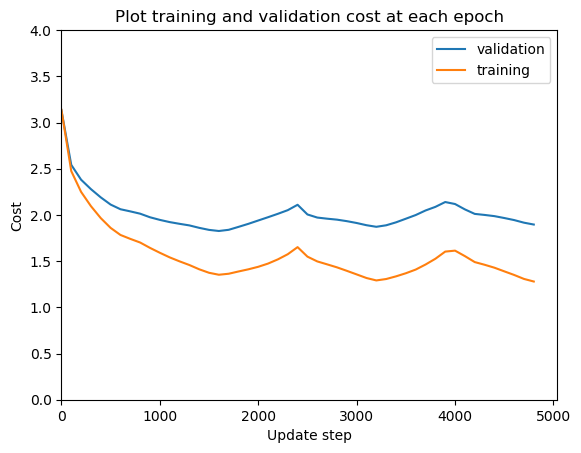
\includegraphics[width=\linewidth]{f4_cost_plt.png}
        \caption{Cost plot}
    \end{subfigure}
    \hfill
    \begin{subfigure}[b]{0.32\textwidth}
        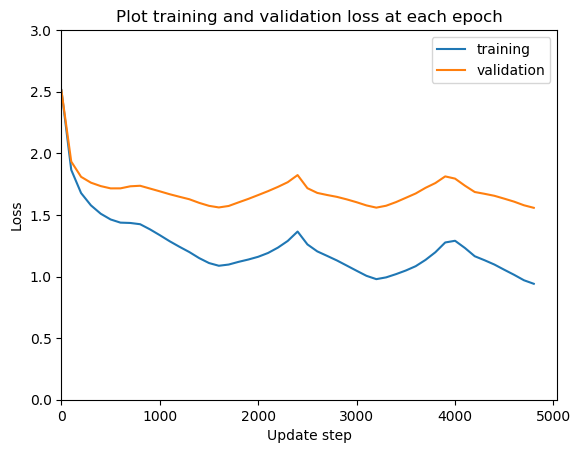
\includegraphics[width=\linewidth]{f4_loss_plt.png}
        \caption{Loss plot}
    \end{subfigure}\hfill
    \begin{subfigure}[b]{0.32\textwidth}%
        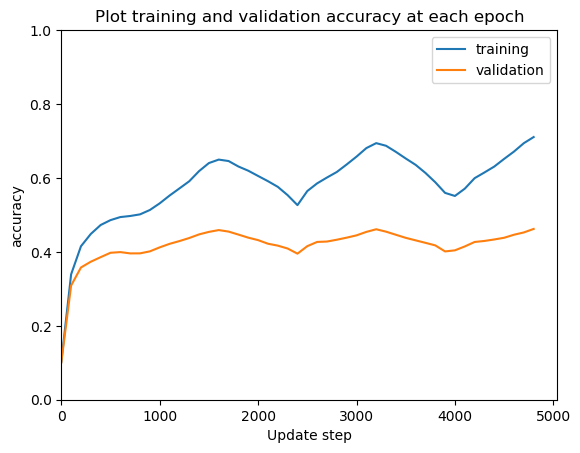
\includegraphics[width=\linewidth]{f4_acc_plt.png}
        \caption{Accuracy plot}
    \end{subfigure}
    \caption{
        Training with default parameters for three cycle:
        \texttt{eta\_min = 1e-5, eta\_max = 1e-1,  lambda = .01 and n\_s = 800}
    }
    \label{fig:replicate_f4}
\end{figure}
\end{question}

\begin{question}{iii}
The best 3 networks and their lambda values and their accuracy on the validation
set are stated in the table \ref{table:coarse_search_lambda}.

In the coarse search, the search range of the lambda value was from $10^{-5}$
to $10^{-1}$. Two cycles were trained. The step size (\texttt{n\_s})
of the cyclic learning rate was 900. The maximum value and the minimum of the
learning rate were \texttt{1e-1} and \texttt{1e-5} respectively. The
\texttt{n\_batch} is 100.

\begin{table}
    \centering
    \begin{tabular}{|c|c|}
    \hline
    lambda value & validation score \\ \hline
    0.003039 & 0.522867    \\ \hline
    0.000083 & 0.520333    \\ \hline
    0.000534 & 0.519867    \\ \hline
    \end{tabular}
    \caption{The 3 best networks and their lambda values in the coarse search}
    \label{table:coarse_search_lambda}
\end{table}
\end{question}

\begin{question}{iv}
    The best 3 networks and their lambda values and their accuracy on the validation
    set are stated in the table \ref{table:fine_search_lambda}.

    In the fine search, the search range of the lambda value was from $10^{-5}$
    to $10^{-3.5}$. Three cycles were trained. The step size (\texttt{n\_s})
    of the cyclic learning rate was 1350. The maximum value and the minimum of the
    learning rate were \texttt{1e-1} and \texttt{1e-5} respectively. The
    \texttt{n\_batch} is 100.

    \begin{table}
        \centering
        \begin{tabular}{|c|c|}
        \hline
        lambda value & validation score \\ \hline
        0.000142 & 0.519533    \\ \hline
        0.000182 & 0.518667    \\ \hline
        0.000062 & 0.517467    \\ \hline
        \end{tabular}
        \caption{The 3 best networks and their lambda values in the fine search}
        \label{table:fine_search_lambda}
    \end{table}
\end{question}

\begin{question}{v}
The best \texttt{lambda} was 0.000142 which was found in the fine search.

The parameter settings were the same as the fine search. The network with the
parameter settings was trained three times. The test accuracy for the three trainings
were 0.5123, 0.5091 and 0.5133.
The cost, loss, and the accuracy during the training process of best performed network
(with the test accuracy 0.5133) were plotted in figure \ref{fig:best_lambda}.

\begin{figure}[!htb]
    \begin{subfigure}[b]{0.32\textwidth}
        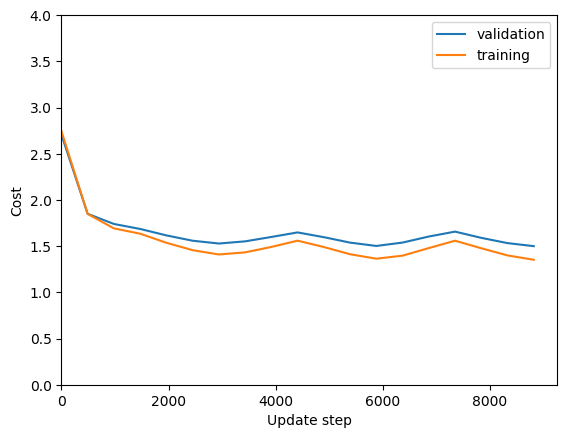
\includegraphics[width=\linewidth]{f5_cost_plt.png}
        \caption{Cost plot}
    \end{subfigure}
    \hfill
    \begin{subfigure}[b]{0.32\textwidth}
        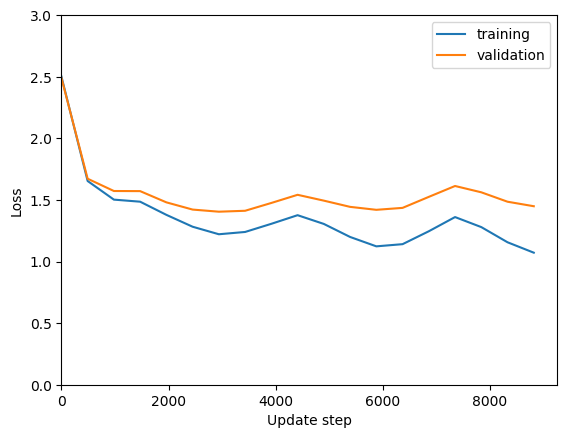
\includegraphics[width=\linewidth]{f5_loss_plt.png}
        \caption{Loss plot}
    \end{subfigure}\hfill
    \begin{subfigure}[b]{0.32\textwidth}%
        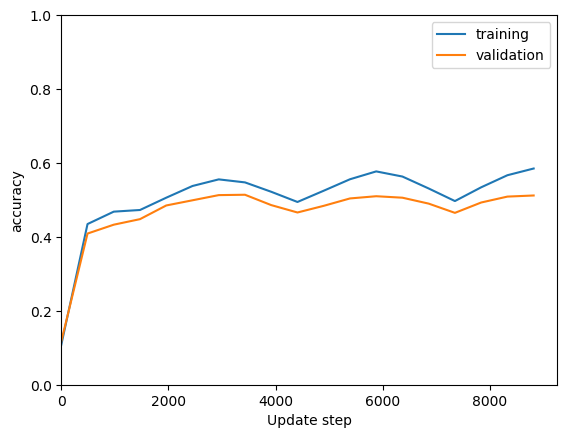
\includegraphics[width=\linewidth]{f5_acc_plt.png}
        \caption{Accuracy plot}
    \end{subfigure}
    \caption{
        The training process of the best performed network with the parameters:
        \texttt{eta\_min = 1e-5, eta\_max = 1e-1,  lambda = .01 and n\_s = 1500}.
        Three training cycles were performed.
    }
    \label{fig:best_lambda}
\end{figure}
\end{question}

\end{document}
